\chapter{Resultados} \label{cap:resultados}

\TEXTO{Este capítulo descreve os principais resultados experimentais obtidos durante esta pesquisa. Como descrito no capítulo anterior, os experimentos foram conduzidos em duas fases. Contudo, optou-se por apresentar, neste capítulo, apenas os principais resultados obtidos. Um sumário dos demais resultados estão disponíveis no Anexo XX deste documento.}

\TEXTO{Antes de apresentar os resultados, as primeiras seções introduzem a organização dos dados, um breve análise das variáveis e o protocolo experimental, respectivamente.}

\section{Organização do conjunto de dados}
\TODO{descrever, nessa seção, como os dados foram organizados em treino, validação e teste}

    O procedimento de coleta de dados foi realizado de acordo com a metodologia da subseção \ref{subsec:coleta_endogenos} para os dados endógenos, e de acordo com os passos da subseção \ref{subsec:coleta_exógenos} foram obtidos os dados exógenos. 
    Ambos os conjuntos de dados coletados foram estruturados conforme a tabela \ref{table:dataset_final}, contendo um intervalo temporal de registros, desde a data 2017-04-12 (12 de abril de 2017) para o primeiro registro até a data 2019-12-16 (16 de dezembro de 2019) para o último registros, totalizando 514 registros de consumo de refeições em dias letivos.
    
    Conforme a metodologia definida na subseção \ref{subsec:fases_experimentais} este conjunto de dados com o total de 514 registros, foi duplicado para 2 fases experimentais distintas, cada uma com sua organização específica do conjunto de dados.
    
    O conjunto de dados da primeira fase experimental foi organizado de acordo com a figura \ref{fig:case1_timeline}, esta fase tem o conjunto de validação contemplando exclusivamente o primeiro semestre de 2018, indicando uma hipótese de que o primeiro semestre de 2018 tivesse um movimento de consumo e vendas semelhantes ao primeiro semestre de 2019, tal que esta fase seria a ideal para testes envolvendo só o primeiro semestre do conjunto de testes.

    \begin{figure}[htb]
        	\center{
        		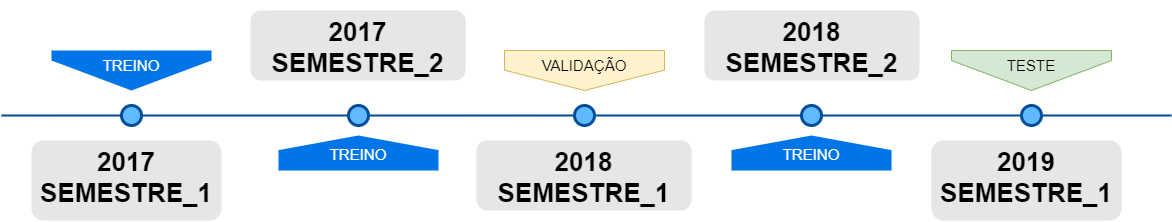
\includegraphics[width=1.0\textwidth]{./Figuras/resultados/case1_timeline.png}
        	
        	\caption{Domínio temporal da 1a fase} \label{fig:case1_timeline} }
        \end{figure}
    E na segunda fase o conjunto de dados foi organizado de acordo com a figura \ref{fig:case2_timeline}, e como esta fase teve um conjunto de validação contemplando 1 ano letivo inteiro, o de 2018, os experimentos de testes dos modelos nesta fase contemplaram o ano todo de 2019.
    
    \begin{figure}[H]
        	\center{
        		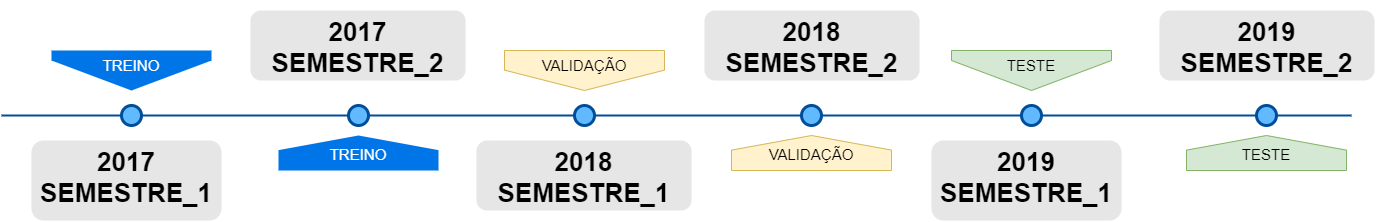
\includegraphics[width=1.0\textwidth]{./Figuras/resultados/case2/case2_dominio.png}
        	
        	\caption{Domínio temporal da 2a fase} \label{fig:case2_timeline} }
        \end{figure}
   
    \paragraph{Dificuldades encontradas e resolvidas}
    A primeira dificuldade encontrada nos experimentos foi um comportamento anômalo do gráfico de previsão, a linha azul na figura \ref{fig:pandas_wrong_indexing} representa uma previsão do modelo que obteve os melhores resultados na primeira fase, e a linha vermelha neste mesmo gráfico representando os valores reais de consumo do primeiro semestre de 2019 também foi anômala. E após uma análise foi descoberto que os registros continham um erro na indexação por data, trocando datas (dia por mês e mês por dia), após a correção da indexação os gráficos de consumo real e previsão produziram resultados melhores e dentro do formato esperado, conforme a figura \ref{fig:pandas_correct_indexing}.
    
    \begin{figure}[htb]
    	\center{
    		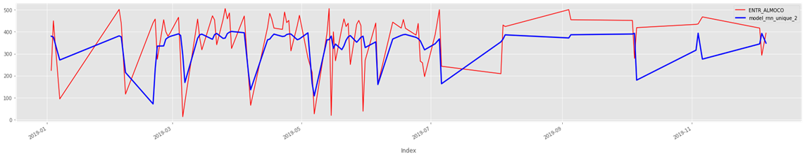
\includegraphics[width=1.0\textwidth]{./Figuras/resultados/pandas_wrong_indexing.png}
    	
    	\caption{Resultado do modelo RNN\_ENDO\_2 obtido sobre o conjunto de dados aleatoriamente ordenado sobre o tempo} \label{fig:pandas_wrong_indexing} }
    \end{figure}
    
    \begin{figure}[htb]
    	\center{
    		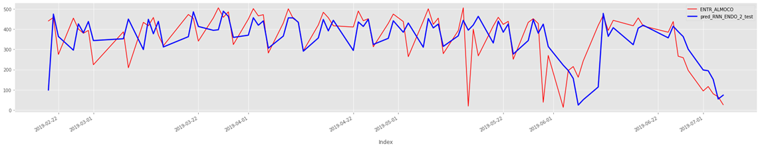
\includegraphics[width=1.0\textwidth]{./Figuras/resultados/pandas_correct_indexing.png}
    	
    	\caption{Resultado do modelo RNN\_ENDO\_2 obtido sobre o conjunto de dados com ordenação corrigida \label{fig:pandas_correct_indexing} }}
    \end{figure}
              
\section{Avaliação das Variáveis}
\TODO{use essa seção se quiser detalhar algo sobre as principais variáveis consideradas, caso contrário, pode excluí-la. Ajuste o texto inicial do capítulo se resolver remover essa seção}

    \paragraph{Estimativas de consumo do restaurante}
        A análise da técnica de estimação de consumo, realizada pela análise subjetiva do consumo da semana anterior, foi feita com o cálculo de 30\% de produção acima do consumo do 5o dia anterior. É possível notar que este método de estimativa é feito para tolerar descartes devido à multa contratual para falta de refeições e que a produção de 30\% de refeições acima do consumo da semana anterior, na figura  \ref{fig:ru_pred} produz um comportamento linear, na linha azul, distante do comportamento real de consumo na linha vermelha. Apesar da estimativa seguir as tendências de quedas e aumento de consumo, a figura \ref{fig:ru_pred_scatter} do gráfico scatter gerado entre a estimava do R.U e o consumo real no ano de 2019, demonstra que a regressão linear (representada pela linha vermelha no gráfico scatter) tem o eixo totalmente descentralizado com a função identidade da estimativa ideal (representada pela diagonal imaginária formada entre a origem do gráfico e o vértice superior direito), gerando também um erro maior do que 30\% no somatório total de refeições descartadas no semestre, ocasionado pelo comportamento oscilatório do consumo, conforme a tabela \ref{table:case2_rupred}.
        {
            \begin{center}
            \begin{minipage}[c]{1.0\textwidth}
                \begin{figure}[H]
                    \center{                    
                        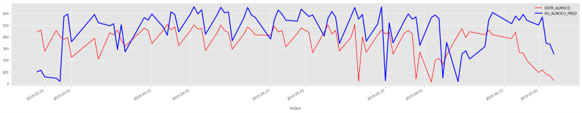
\includegraphics[width=\textwidth]{./Figuras/resultados/case1_ru_pred.png}
                        \caption{Estimativa do restaurante para o ano de 2019} \label{fig:ru_pred} 
                    }
                \end{figure}
            \end{minipage} \hfill %
            
            \begin{minipage}[c]{0.8\textwidth}
                \begin{figure}[H]
                    \center{                    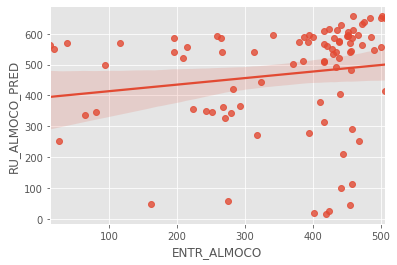
\includegraphics[width=\textwidth]{./Figuras/resultados/case1_ru_pred_scatter.png}
                    \caption{Gráfico scatter da estimativa de consumo do restaurante para o ano de 2019} \label{fig:ru_pred_scatter} }
                \end{figure} 
            \end{minipage} 
            \end{center}
            
            \begin{table}[!ht]
            \centering
            \caption{Métricas da estima de consumo do restaurante para o ano de 2019}
            \label{table:case2_rupred}
            \rowcolors{2}{gray!25}{white}
                \begin{tabular}{|c|c|}
                \rowcolor{gray!50}
                \hline
                \multicolumn{2}{c}{Consumo com margem 30\% acima do 5o dia anterior}\\ \hline     
                TOTAL DE REFEIÇÕES CONSUMIDAS & 58653  \\
                TOTAL DE REFEIÇÕES ESTIMADAS & 76262 \\ 
                CORRELAÇÃO (r)&  0.40067947341844423 \\
                P-value & 2.0845891721642294e-08\\
                RMSE & 191.7620291511743 \\
                SOMA DOS ERROS POSITIVOS & 23412 \\
                SOMA DOS ERROS NEGATIVOS & -5803 \\
                ERRO ABSOLUTO MEDIANO & 133.0 \\
                ERRO ABSOLUTO PERCENTUAL MEDIO & 205.61135949728225\% \\  \hline 
                \end{tabular}
            \end{table}
        }
    \subsection{Análise das variáveis endógenas}
        As variáveis endógenas são os parâmetros temporais de entrada nos modelos MLP e GRU, correspondentes ao domínio de consumo no restaurante.
         % \newpage
        \paragraph*{Consumo do dia vigente em relação às vendas de tickets do dia anterior}
        É possível notar na figura \ref{fig:case1_consumo_vendas_almoco} que as vendas de ticket no período de almoço apresentaram comportamento diferente no ano de 2017 em comparação aos anos seguintes devido à uma limitação imposta pelo restaurante, a partir de 2018, que os alunos comprassem apenas 2 tickets por dia. Possivelmente esta limitação foi dada para aproximar o comportamento de consumo de 1 até 2 dias seguintes à vendas de tickets no dia vigente, esta limitação pode ser interpretada como método de auxílio à gestão para a produção de refeições e para o tratamento de desperdício.
	        
        Mesmo com o valor outlier de 2000 vendas em um único dia, e com a nova limitação de compras de tickets a partir de 2018, o consumo no horário de almoço está fortemente relacionado com as vendas de tickets no período do almoço de 1 dia anterior e nota-se que os alunos se adaptaram à limitação imposta para utilização dos tickets com prazo de validade de 2 dias, conforme o valor de correlação aproximado em 72\% que pode ser conferido na tabela \ref{table:case1_vendas1}.
        
        Há outros fatores não previstos envolvidos, como possíveis falha de registros de vendas no sistema, bem como o outlier de 2000 vendas pode ser interpretado com a migração de sistema e banco de dados de refeições que ocorreu em 2017 da unidade talim do ICT Unifesp para o banco de dados do Hospital São Paulo, possivelmente também foram importadas vendas do sistema antigo sem a diferenciação de datas. A soma de vendas de tickets no horário do almoço, totalizou 242282 tickets vendidos no período do almoço, em todo o conjunto de dados de 514 registros, e a soma de passagens de alunos pela catraca do restaurante também no período do almoço, sendo o valor real de consumo, totalizou 163752 refeições. Apesar de notória a diferença de 78.530 tickets vendidos acima do consumo real não foi possível investigar neste trabalho as causas desta diferença, ressaltando que estes valores foram obtidos no conjunto original de dados fornecidos pelo fiscal de contrato do R.U do ICT Unifesp através de consulta solicitada via e-mail para este fiscal.

	       {
	       \begin{center} 
    	        \begin{minipage}[c]{1.0\textwidth}
    	            \begin{figure}[H]
                    	\center{                    		        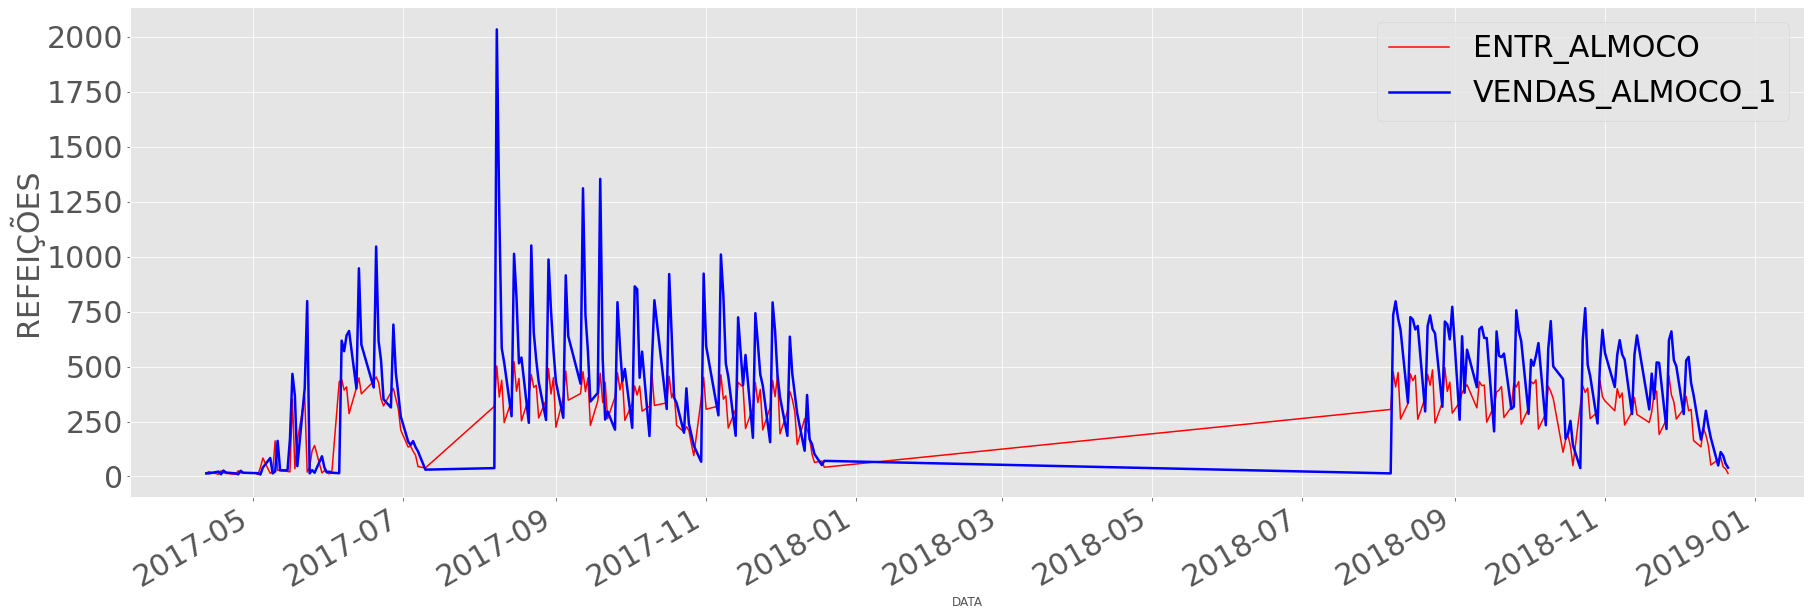
\includegraphics[width=1.0\textwidth]{./Figuras/resultados/case1_consumo_vendas_almoco.png}
                    	\caption{Correlação entre consumo e vendas de almoço.} \label{fig:case1_consumo_vendas_almoco} 
                    	}
                    \end{figure}
                \end{minipage} \hfill %
                \begin{minipage}[c]{0.3\textwidth}
                    \begin{figure}[H]
                    	\center{                    		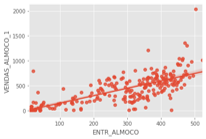
\includegraphics[width=1.0\textwidth]{./Figuras/resultados/case1_scatter_consumo_vendas_almoco.png}
                    	\caption{Gráfico Scatter entre consumo e vendas de almoço.} \label{fig:case1_scatter_consumo_vendas_almoco} }
                    \end{figure}
                \end{minipage} 
            \end{center}
            }
                
           \begin{table}[!ht]
           \centering
           \caption{Comparação de consumo com um dia anterior}
             \rowcolors{2}{gray!25}{white}
             \begin{tabular}{|c|c|}\hline
                \multicolumn{2}{c}{CONSUMO EM RELAÇÃO ÀS VENDAS DE 1 DIA ANTERIOR}\\ \hline
                CORRELAÇÃO (r) &  0.7255528038157009\\
                P-value &5.399561176138223e-41\\
                RMSE & 260.5399426736619\\
                TOTAL DE REFEIÇÕES PROJETADAS & 104694\\ 
                TOTAL DE REFEIÇÕES CONSUMIDAS & 69544\\
                TOTAL DE REFEIÇÕES SUB PROJETADAS & -4703\\
                TOTAL DE REFEIÇÕES SUPER PROJETADAS & 39853\\
                ERRO ABSOLUTO MEDIANO & 139.0\\
                ERRO ABSOLUTO PERCENTUAL MEDIO & 90.18\\\hline
            \end{tabular} \label{table:case1_vendas1} \end{table}

            \paragraph*{Normalização e escala de features}
                O processo de normalização e escala é demonstrado nesta seção com a feature de vendas de tickets de 1 dia anterior, pois entre todas as features esta é a que produziu outliers com maior destaque.
                A normalização dos dados é feita com o teto de 3x o desvio padrão médio, logo o pico de 2000 vendas foi normalizado para o valor arredondado de 1356 refeições e mesmo com a normalização, o comportamento linear desta feature, conforme figura \ref{fig:feature_sem_outliers}, se manteve.   
                E após a normalização foi realizada a aplicação da escala de 0 a 1 na feature e conforme é observado na figura  \ref{fig:feature_sem_outliers_escalada}, o comportamento linear da feature também se manteve.

                {
                    \begin{center}
                        \begin{minipage}[b]{1.0\textwidth}
                        \begin{figure}[H]
                        	\center{
                            	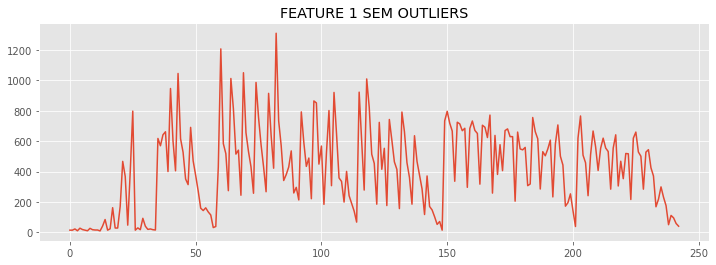
\includegraphics[width=1.0\textwidth]{./Figuras/resultados/feature_sem_outliers.png}
                            	\caption{Vendas de tickets normalizados com teto de 3x o desvio padrão.}
                            	\label{fig:feature_sem_outliers}
                        	}
                        \end{figure}
                        \end{minipage} \hfill %
                        
                        \begin{minipage}[b]{1.0\textwidth}
                        \begin{figure}[H]
                        	\center
                        	{                    		
                            	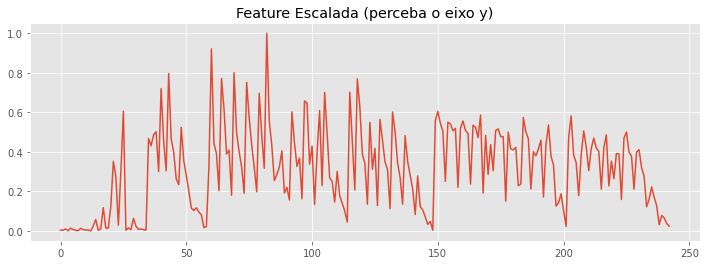
\includegraphics[width=1.0\textwidth]{./Figuras/resultados/feature_sem_outliers_escalada.png}
                            	\caption{Vendas de tickets escalada entre 0 a 1.} \label{fig:feature_sem_outliers_escalada} 
                        	}
                        \end{figure}
                        \end{minipage}
                    \end{center}
                }
                Este processo de normalização e escala foi realizado para todas as features endógenas e para as features climáticas.
        	   % \newpage
        	   
                \paragraph{Consumo atual em relação ao consumo do jantar de 1 dia anterior.}
                
                    Apesar de que os alunos que consomem refeições no almoço geralmente são de período e de grade horária diferente dos alunos que consomem o jantar no período da noite, nota-se uma relação evidente entre os 2 consumos, evidenciada pelo comportamento linear na figura \ref{fig:case1_consumo_jantar} com correlação (r) = 0.7655, e pela regressão linear entre esses 2 consumos na figura  \ref{fig:case1_consumo_jantar_scatter}, não foi possível encontrar uma causa evidente para este efeito anômalo.
                    
                    {\begin{center} 
                    \begin{minipage}[c]{1.0\textwidth}
                    \begin{figure}[H]
                    	\center{
                    	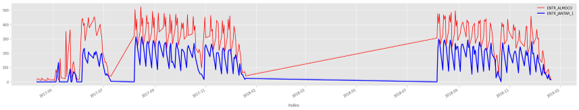
\includegraphics[width=1.0\textwidth]{./Figuras/resultados/case1_consumo_jantar.png}
                    	\caption{Correlação de consumo de almoço e jantar de 1 dia anterior.} 
                    	\label{fig:case1_consumo_jantar} }
                    \end{figure} 
                    \end{minipage}\hfill %
                    
                    \begin{minipage}[c]{0.3\textwidth}
                    \begin{figure}[H]
                    	\center{                    		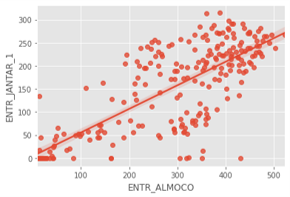
\includegraphics[width=1.0\textwidth]{./Figuras/resultados/case1_consumo_jantar_scatter.png}
                    	\caption{Gráfico Scatter entre consumo e jantar de 1 dia anterior.} 
                    	\label{fig:case1_consumo_jantar_scatter} }
                    \end{figure}
                    \end{minipage} \end{center} }
            
    	    \paragraph{Análise da sazonalidade semanal}
    	        Os gráficos de consumo a seguir da figura  \ref{fig:case1_violinplot_segunda}, representando a segunda-feira,  até a figura \ref{fig:case1_violinplot_sexta} , representando a sexta-feira,  são gerados para as features categóricas binárias, com a funcionalidade violin-plot da biblioteca seaborn, própria para distribuição de variáveis categóricas-binárias em um dataset.
    	        O violino azul com o valor 1 representa a distribuição do consumo ao longo do conjunto total de dados.
    	        O violino com valor zero pode ser ignorado e é um retorno padrão no gráfico da ferramenta, representando o complemento do consumo para o dia da semana considerado.
    	        Nas sextas feiras, o consumo teve escala de distribuição menor para todo o conjunto 2019. Foi notório que apesar da alternância de grades horárias durante a troca de semestres no ano de 2019, os dias de terça e quinta feira concentraram o maior movimento de consumo.
    	       %\newpage
    	       \begin{center}    
    	        \begin{minipage}[c]{0.45\textwidth}
    	         \begin{figure}[H]
                	\center{                		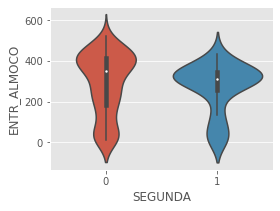
\includegraphics[width=\textwidth]{./Figuras/resultados/case1_segunda.png}
                	\caption{Gráfico violino da distribuição do consumo na segunda feira.} \label{fig:case1_violinplot_segunda} }
                \end{figure}\end{minipage} \hfill %
                      \begin{minipage}[c]{0.45\textwidth}
                \begin{figure}[H]
                	\center{                		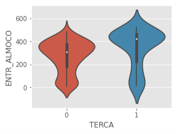
\includegraphics[width=\textwidth]{./Figuras/resultados/case1_terca.png}
                	\caption{Gráfico violino da distribuição do consumo na terça feira.} \label{fig:case1_violinplot_terca} }
                \end{figure} \end{minipage}
                 \begin{minipage}[c]{0.45\textwidth} 
                \begin{figure}[H]
                	\center{                		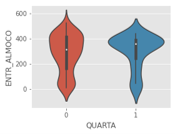
\includegraphics[width=\textwidth]{./Figuras/resultados/case1_quarta.png}
                	\caption{Gráfico violino da distribuição do consumo na quarta feira.	} \label{fig:case1_violinplot_quarta} }
                \end{figure}\end{minipage} \hfill %
                      \begin{minipage}[c]{0.45\textwidth}
                \begin{figure}[H]
                	\center{                		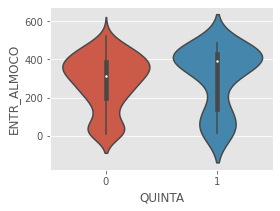
\includegraphics[width=\textwidth]{./Figuras/resultados/case1_quinta.png}
                	\caption{Gráfico violino da distribuição do consumo na quinta feira.} \label{fig:case1_violinplot_quinta} }
                \end{figure}\end{minipage} %
                        \begin{minipage}[c]{0.45\textwidth}
                \begin{figure}[H]
                	\center{                		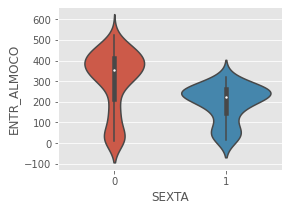
\includegraphics[width=\textwidth]{./Figuras/resultados/case1_sexta.png}
                	\caption{Gráfico violino da distribuição do consumo na sexta feira.} \label{fig:case1_violinplot_sexta} }
                \end{figure}
                \end{minipage} \end{center}
    \subsection{Análise das variáveis exógenas}
        As variáveis exógenas correspondem aos parâmetros, de domínio discreto, que são utilizados exclusivamente nos modelos de redes neurais mistos, e são lidos pelas camadas MLP destes modelos.
        \paragraph{Consumo atual em relação ao avanço do semestre}
        Para esta análise foi necessário restringir o domínio de análise para 1 semestre, o consumo em relação ao avanço do semestre teve queda abrupta nos ultimos dias do semestre, portanto a correlação dos conjuntos de dados das figuras \ref{fig:case1_perc_sem} e \ref{fig:case1_perc_sem_scatter} obteve valor negativo.
        {
        \begin{center} 
        
            \begin{minipage}[c]{1.0\textwidth}
                \begin{figure}[H]
                	\center{                    		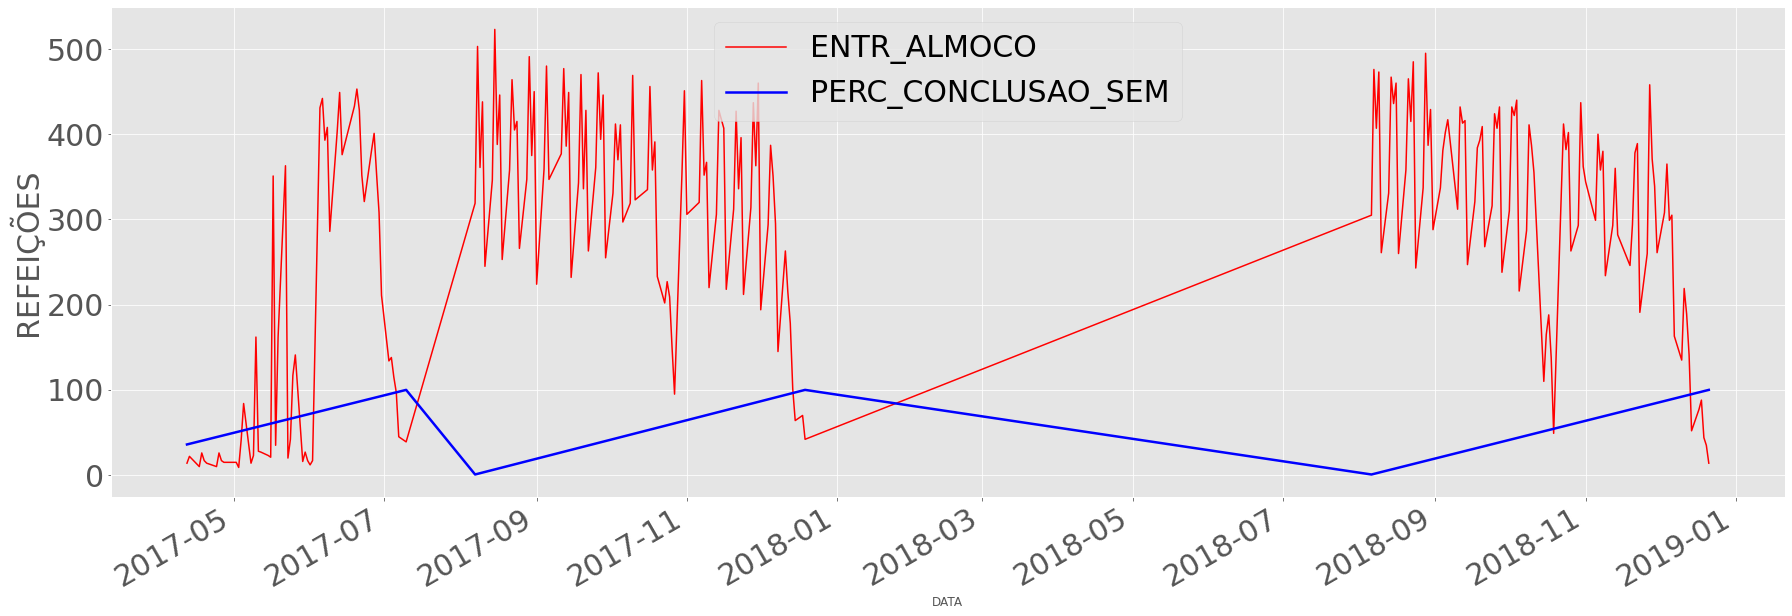
\includegraphics[width=\textwidth]{./Figuras/resultados/case1_perc_sem.png}
                	\caption{1a Fase : Relação da distribuição do consumo com o avanço do semestre, Correlação (r) = -0.35}
                	\label{fig:case1_perc_sem}
                	}
                \end{figure}  
            \end{minipage} \hfill %
        
            \begin{minipage}[c]{0.5\textwidth}
                \begin{figure}[H]
                	\center{                		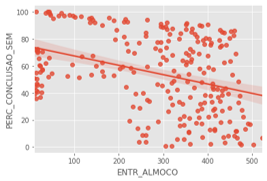
\includegraphics[width=\textwidth]{./Figuras/resultados/case1_perc_sem_scatter.png}
                	\caption{Gráfico scatter da distribuição do consumo com o avanço do semestre.} \label{fig:case1_perc_sem_scatter}
                	}
                \end{figure}
            \end{minipage} 
        \end{center} 
        }

\section{Protocolo Experimental}
\TODO{faça um resumo sobre as duas fases e as principais diferenças entre elas. Na sequência, detalhe os detalhes do principal modelo obtido (o com melhor resultado de predição)}
    
    \subsection{Avaliação do aprendizado do problema da predição de refeições por meio de redes neurais MLP}
        \paragraph{Ajuste empírico de topologia do primeiro modelo perceptron}
        O primeiro experimento com redes neurais realizado na primeira fase experimental, avaliou a capacidade de aprendizado do modelo perceptron sobre a sazonalidade dos dados endógenos, referentes ao domínio de consumo de refeições no R.U, verificando se o comportamento de consumo no restaurante pôde ser aprendido por este tipo de rede neural, portanto foi definida 1 rede neural inicial perceptron com apenas 1 camada oculta contendo 1 neurônio para 15 parâmetros de entrada (mesmo número de parâmetros endógenos) e com 1 neurônio de saída, denominada de MLP1.
        
        Os parâmetros endógenos correspondem à uma série temporal de intervalo de 5 dias anteriores para consumo de refeições no período do almoço, jantar e de vendas de tickets no período do almoço.
        O modelo foi denominado MLP1, sua ilustração pode ser visualizada na figura \ref{fig:case1_mlp1} obtida através da ferramenta NETRON. Cada camada do modelo MLP1 corresponde à um bloco com título \textbf{Dense} nesta figura, a primeira aresta da figura entre o bloco input e InputLayer demonstra as 3 séries temporais dos parâmetros de entrada, com intervalo de 5 dias passados cada. \textbf{ENTR\_ALMOCO, ENTR\_JANTAR e VENDAS\_ALMOCO}. O bloco Flatten converte cada dia de entrada das séries temporais em um parâmetro de entrada da rede neural MLP, conforme modelo conceitual do trabalho de \citeonline{Lopes2008} ilustrado na figura \ref{fig:mlp-lopes} que utiliza apenas 1 parâmetro endógeno com intervalo temporal também de 5 dias. A primeira camada oculta desta rede pode ser visualizada no primeiro bloco dense da figura que demonstra a função de ativação ReLu deste neurônio, e o número de unidades desta camada sendo 1.
        A camada de saída é o último bloco da figura, também com 1 unidade, e como a função de ativação é linear, ela não é exibida na descrição do bloco.
        \begin{figure}[H]
        \center{
        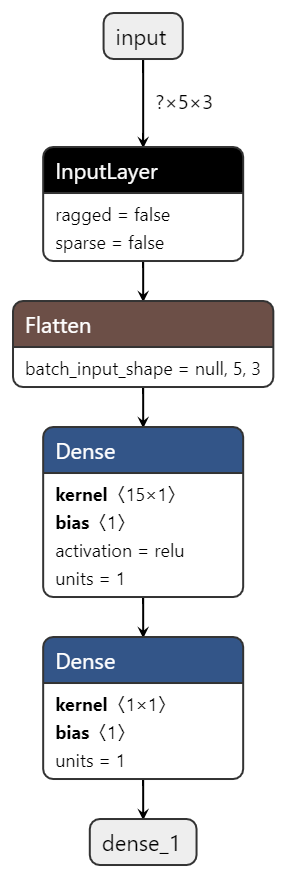
\includegraphics[width=0.3\textwidth]{./Figuras/resultados/case1_MLP1_validated.png}
        	\caption{Topologia do modelo MLP1, Ferramenta NETRON} 
        	\label{fig:case1_mlp1}
        }
        \end{figure}
        O treino deste modelo foi executado, obtendo RMSE com o valor 130,62 sobre o conjunto de validação, neste caso da primeira fase sendo os dados do primeiro semestre de 2018, e é possível notar figura \ref{fig:case1_mlp1_train} que as linhas da função de perda e treino convergiram à um processo de overfitting e não demonstraram aprendizado significante deste modelo sobre o conjunto de validação.
        \begin{figure}[H]
        	\center{
        	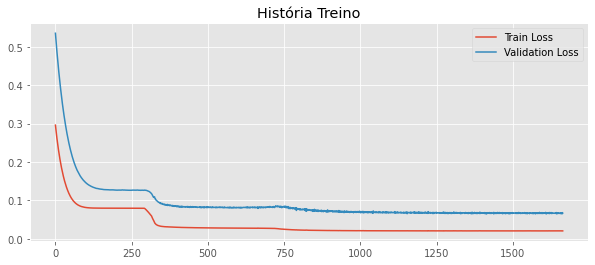
\includegraphics[width=0.8\textwidth]{./Figuras/resultados/case1_mlp1_train.png}
        	\caption{Gráfico de treino do modelo MLP1, RMSE = 130,62}
        	\label{fig:case1_mlp1_train}
        	}
        \end{figure}
        
        Portanto foi aumentada a profundidade do modelo MLP1 obtendo-se o modelo MLP2 com topologia ilustrada na figura  \ref{fig:case1_mlp2}, e após o treino deste modelo foi possível notar a diminuição do RMSE (Raiz do erro quadrático médio) para o valor de 107.97, observado na figura \ref{fig:case1_mlp2_train}. Validando a hipótese de que a predição do consumo no restaurante, pode ser aprendida por modelos simples de redes neurais, e portanto a pesquisa seguiu com a definição de novos modelos demonstrados na próxima subseção.
        \begin{figure}[H]
        	\center{
        		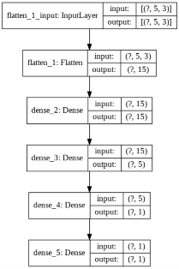
\includegraphics[width=0.3\textwidth]{./Figuras/resultados/case1_mlp2.png}
        	\caption{Topologia do modelo MLP2} \label{fig:case1_mlp2} }
        \end{figure}
        \begin{figure}[H]
        	\center{
        		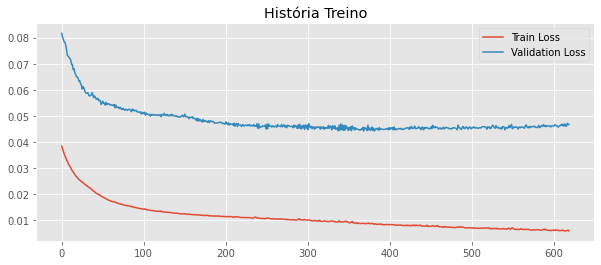
\includegraphics[width=1.0\textwidth]{./Figuras/resultados/case1_mlp2_train.png}
        	\caption{Gráfico de treino do modelo MLP2. RMSE = 107.97}
        	\label{fig:case1_mlp2_train} }
        \end{figure}
    \subsection{Definições das topologias dos modelos}
        \paragraph{Modelo endógeno MLP\_ENDO\_1}
            O primeiro modelo experimental MLP para obtenção das predições tem topologia definida na figura \ref{fig:case1_mlp_endo1}, denominado MLP\_ENDO\_1, este modelo tem 64 neurônios na primeira camada oculta e 32 neurônios na segunda camada oculta, e assim como todos os outros modelos, 1 neurônio na camada de saída. Ressaltando que a metodologia do cap \ref{cap:metodos} define que para os modelos MLP as camadas ocultas utilizam função de ativação ReLu e função de saída Linear.
            \begin{figure}[H]
            	\center{                		
            	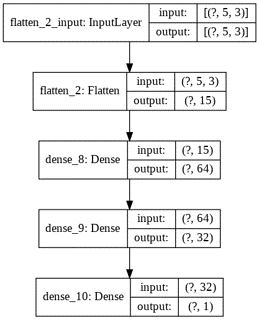
\includegraphics[width=0.25\textwidth]{./Figuras/resultados/case1_mlp_endo1.png}
            	\caption{Topologia do modelo MLP\_ENDO\_1} 
            	\label{fig:case1_mlp_endo1} 
            	}
            \end{figure}
            
         \paragraph{Modelo endógeno GRU RNN\_ENDO\_1}
            Este primeiro modelo experimental GRU foi definido com 16 unidades GRU, com topologia conceitual definida de acordo com a figura \ref{fig:gru-arch} no capítulo de fundamentação teórica \textbf{MLP\_ENDO\_1} e tem um neurônio perpcetron para emissão do sinal de saída, representado pelo bloco\textbf{Dense} na figura \ref{fig:case1_rnn_endo1}
            \begin{figure}[H]
              \center{
                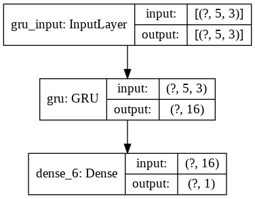
\includegraphics[width=0.25\textwidth]{./Figuras/resultados/case1_rnn_endo1.png}
                \caption{Topologia do modelo RNN\_ENDO\_1} \label{fig:case1_rnn_endo1} }
            \end{figure}
         
         \paragraph{Modelo endógeno GRU RNN\_ENDO\_2}
           Foi definido uma segunda reconfiguração do modelo GRU, RNN\_ENDO\_2, com o aumento da profundidade de unidades do modelo anterior RNN\_ENDO\_1, em formato regressivo de 16 unidades na primeira camada, 8 unidades na segunda e 4 na terceira, e com a inclusão do recurso Dropout entre as unidades para eliminar unidades com pesos negativos no grafo denso da rede, observado na figura \ref{fig:case1_rnn_endo2} realizando a poda de unidades não relevantes durante o treino.
            \begin{figure}[H]
              \center{
                  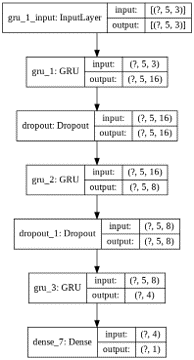
\includegraphics[width=0.20\textwidth]{./Figuras/resultados/case1_rnn_endo2.png}
                  \caption{Topologia do modelo RNN\_ENDO\_2} 
                  \label{fig:case1_rnn_endo2} 
              }
            \end{figure}
        \paragraph{Modelo misto RNN\_EXO\_1}
            Interpretando o digrama do primeiro modelo misto,  \textbf{RNN\_EXO\_1}, na figura \ref{fig:case1_rnn_exo_1}o bloco com título GRU à esquerda na figura de topologia do modelo, trata as entradas endógenas (temporais), assim como exemplificado nos modelos GRU endógenos. O bloco com título \textbf{Dense} é uma rede MLP que recebe um input com 10 parâmetros de 1 dimensão, portanto todos discretos, correspondendo aos 4 parâmetros climáticos (temperatura, umidade, pressão e vento), 1 parâmetro para o dia da semana vigente, 1 para o semestre vigente e 4 parâmetros de controle do calendário (distancia da data anterior, posterior, avanço do semestre, avanço do mês). A saída dos blocos GRU e MLP são concatenadas e tratadas pelo bloco MLP de saída.
            \begin{figure}[H]
              \center{
                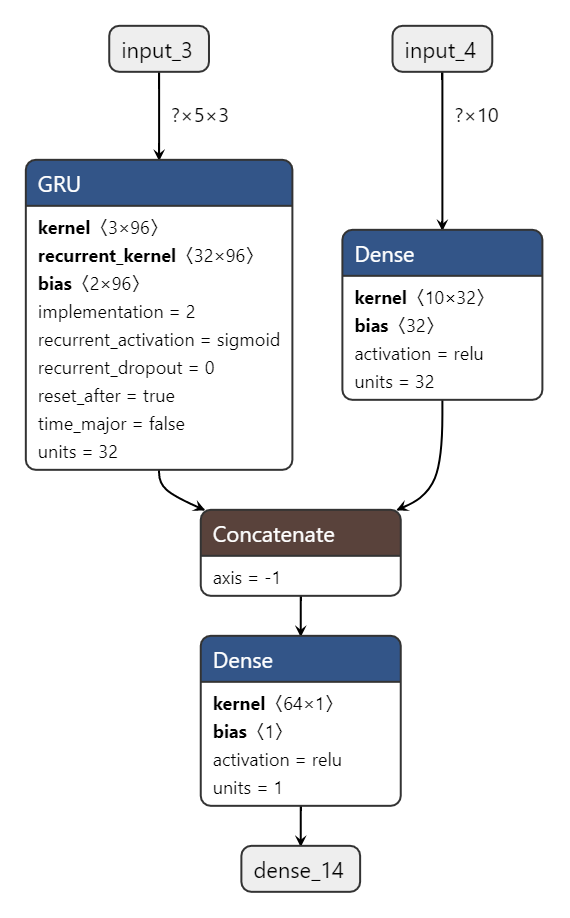
\includegraphics[width=0.7\textwidth]{./Figuras/resultados/case1_rnn_exo_1.png}
                \caption{Topologia do modelo RNN\_EXO\_1} \label{fig:case1_rnn_exo_1} }
            \end{figure}
            
        \paragraph{Modelo misto RNN\_EXO\_2}
         O Segundo modelo misto foi definido com o aumento da profundidade das camadas GRU e MLP do modelo anterior, conforme observado na figura \ref{fig:case1_rnn_exo_2} foram acrescentadas 1 camada GRU e 1 camada MLP (Dense).
            \begin{figure}[H]
              \center{
                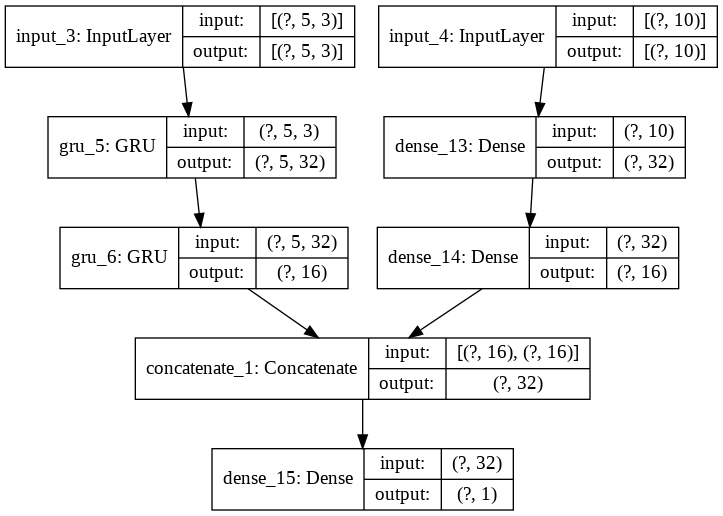
\includegraphics[width=0.6\textwidth]{./Figuras/resultados/case1_rnn_exo_2.png}
              \caption{Topologia do modelo RNN\_EXO\_2}  \label{fig:case1_rnn_exo_2} }
            \end{figure}
        
        \paragraph{Modelo misto RNN\_EXO\_3}
        Para o terceiro e último modelo misto, representado na figura \ref{fig:case1_rnn_exo_3}, foi feita uma reconfiguração do modelo misto anterior com a utilização do recurso dropout nas saídas das camadas GRU, que realiza podas de conexões com pesos negativos.
        \begin{figure}[H]
          \center{
          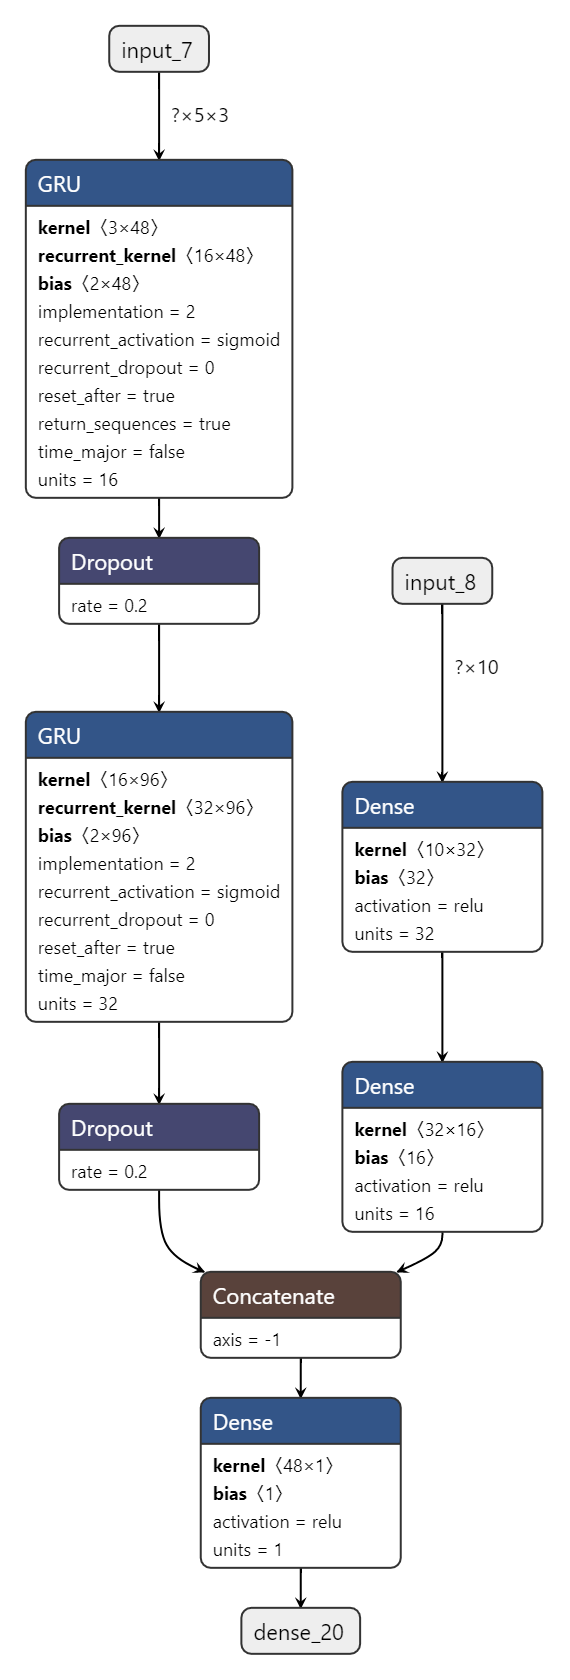
\includegraphics[width=0.5\textwidth]{./Figuras/resultados/case1_rnn_exo_3.png}
          \caption{Topologia do modelo RNN\_EXO\_3} \label{fig:case1_rnn_exo_3} 
          }
        \end{figure}
    \subsection{Diferenças principais dos resultados entre as fases experimentais}
        \paragraph{Diferenças entre os melhores modelos}
        Para os experimentos da 1a fase, o modelo que produziu o menor RMSE no conjunto de testes com vantagem em todas as outras métricas foi o modelo endógeno, RNN\_ENDO\_2, com algumas anomalias de predição observadas na figura \ref{fig:case1_rnn_endo2_test_dates}.
        \begin{figure}[H]
          \center{
            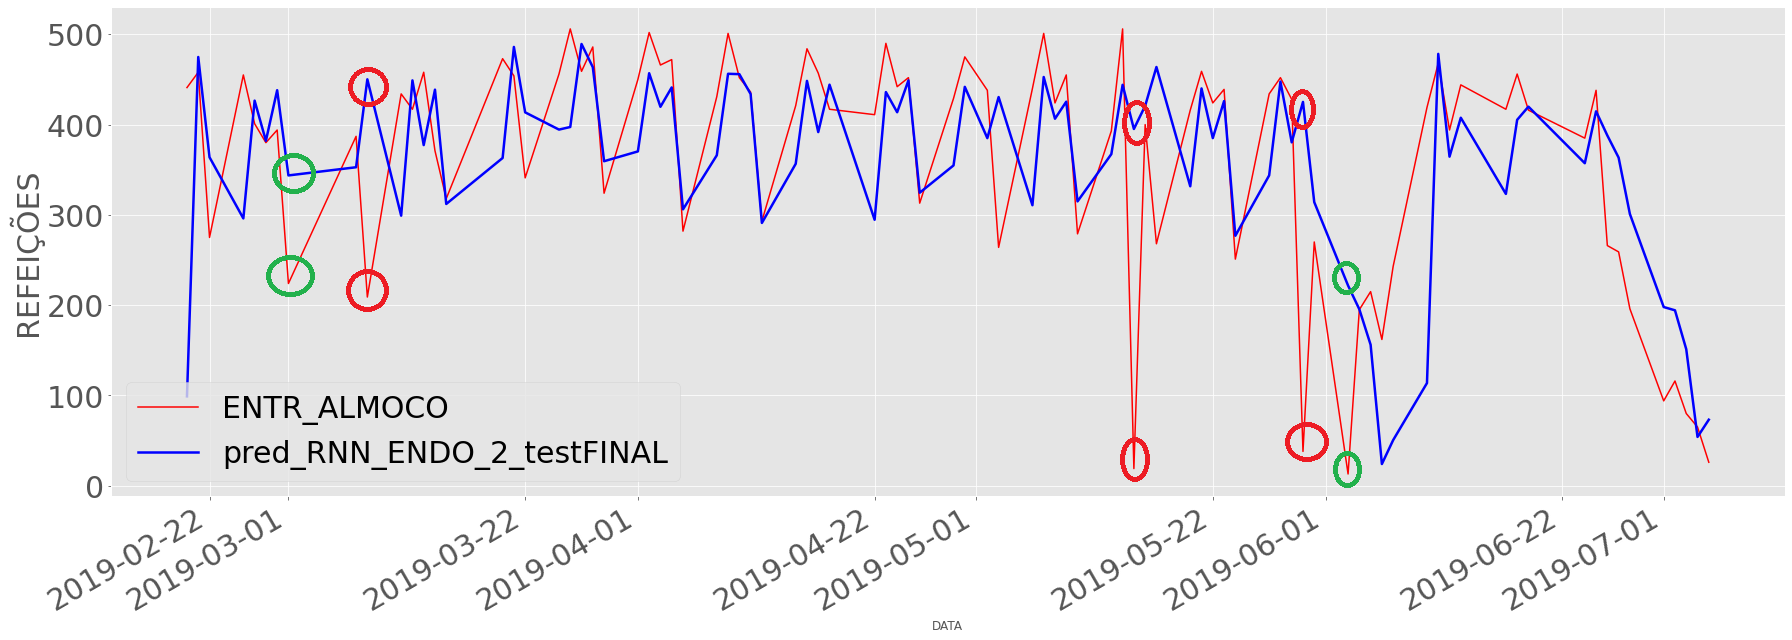
\includegraphics[width=1.0\textwidth]{./Figuras/resultados/case1_rnn_endo2_test_dates.png}
          \caption{Analise de anomalias preditivas do RNN\_ENDO\_2} \label{fig:case1_rnn_endo2_test_dates} }
        \end{figure}
        
        Os pontos verdes outliers representam predições que corresponderam a tendência de alta ou baixa de consumo mas com erros discrepante, e os pontos vermelhos representam predições com tendência inversa ao consumo.
        As justificativas para a predição dentro da tendência, se encontram na tabela \ref{table:rnn_endo_2_green}, denotando datas especiais que não poderiam corresponder ao processo de aprendizado do modelo.
            \begin{table}[!ht]
                \centering
                \caption{Erros de predições do modelo RNN\_ENDO\_2 na 1a fase}
                \label{table:rnn_endo_2_green}
                \rowcolors{2}{gray!25}{white}
                 \begin{tabular}{|c|c|c|}
                 \rowcolor{gray!50}
                 \hline 
                Data & Consumo & Justificativa\\ \hline    
                01/03/2019 (sexta feira)    & 224 & Sexta Feira pré - carnaval\\
                03/06/2019 (segunda feira)  &  13 & Segunda Feira pós paralisação estudantil\\ \hline 
                \end{tabular} 
            \end{table}
            
        As justificativas para previsões onde o modelo seguiu tendência oposta ao consumo também corresponderam à datas especiais, conferidas na tabela \ref{table:rnn_endo_2_red}.
            \begin{table}[!ht]
                \caption{Anomalias de predições do modelo RNN\_ENDO\_2 na 1a fase}
                \label{table:rnn_endo_2_red}
                \rowcolors{2}{gray!25}{white}
                 \begin{tabular}{|c|c|c|}
                 \rowcolor{gray!50}
                 \hline
                Data & Consumo & Justificativa \\
                08/03/2019 (sexta feira)   & 209 &Sexta Feira pós - carnaval\\
                15/05/2019 (quarta feira)   & 19  & Paralisação estudantil na praça Afonso Pena\\
                30/05/2019 (quinta feira)   &  38  & Paralisação estudantil na Praça Afonso pena\\
                \hline 
                \end{tabular} 
            \end{table}
        
        Nas métricas deste modelo, é observado na tabela \ref{table:rnn_endo_2_test} que a soma dos erros positivos, correspondeu à um descarte de aproximadamente 3479 refeiçoes, e o erro quadrático médio de previsão foi de aproximadamente 108 refeições.
            \begin{table}[!ht]
                \centering
                \rowcolors{2}{gray!25}{white}
                \caption{Métricas do melhor modelo:  RNN\_ENDO\_2 }
                \label{table:rnn_endo_2_test}
                \begin{tabular}{|c|c|}
                \rowcolor{gray!50}
                \hline
                Melhor modelo: &   RNN\_ENDO\_2: \\ \hline
                Total\_Consumidas & 31962 \\ 
                Total\_Previstas & 31465,61133 \\
                Erro\_Total\_Previsao & -496,3886719 \\
                Percentual\_Erro\_Total & -1,5530\% \\\
                Correlação & 0,595439895 \\
                P-value & 9,42215E-10    \\
                RMSE &  108,0663015\\
                Soma dos erros Negativos & -2982,567947 \\
                Soma dos erros Positivos & 3478,957266\\
                ERRO\_ABS\_MEDIANO & 46,70721436 \\ 
                ERRO\_ABSOLUTO\_PERCENTUAL\_MEDIO & 74,93539002 \\ 
                \hline
                \end{tabular}
            \end{table}
        
        Já na segunda fase, todos os modelos obtiveram melhoras no erro de treino sobre o conjunto de validação, e foi obtido o modelo com as melhores predições do trabalho, o modelo misto \textbf{RNN\_EXO\_1} detalhado em sua própria seção a seguir.
        É importante notar que as 2 fases produziram melhores modelos de classes distintas, a primeira com um modelo que utiliza apenas dados endógenos, e que contempla um conjunto de validação e teste com amplitude de apenas 1 semestre, e a segunda com um modelo que utiliza dados temporais e discretos, e que utiliza conjunto de validação e teste com amplitude de 1 ano.
        Isso denota que resultados melhores foram conquistados sem nenhuma alteração de parâmetros e hiper-parâmetros nos modelos, alterando-se apenas a organização temporal dos conjuntos de dados.
        
        Durante o teste de todos os modelos, apenas o primeiro semestre contemplou datas especiais onde estes modelos produziram anomalias de previsões, ilustrado como exemplo na figura \ref{fig:case1_rnn_endo2_test_dates}.

\section{Resultados com o Modelo RNN\_EXO\_1}
\TODO{Nessa seção apresente os resultados do melhor modelo. Se quiser, pode dividir em subseções}
    Este modelo, representado na figura \ref{fig:case1_rnn_exo_1} obteve os melhores resultados de todo este trabalho quando foi treinando na segunda fase experimental.
    É notório sua melhoria de resultados com uma única mudança da organização dos conjuntos de dados entre as fases experimentais.
    
    \subsection{Comparativo do treino entre as duas fases}
     Nota-se que este modelo produziu um gráfico função de perda durante o treino, com comportamento oscilatório pior, convergindo mais rapidamente à um overfitting, na primeira fase, ilustrado na figura \ref{fig:case1_rnn_exo_1_train} em comparação ao treino com melhores resultados na segunda fase, ilustrado na figura \ref{fig:case2_rnn_exo1_train}. É notório também a diferença das métricas RMSE entre estes 2 treinos, produzindo um resultado melhor na segunda fase, de RMSE = 109,97 em comparação ao resultado da primeira fase de RMSE = 132,94.
     
     \paragraph{Resultados de treino e validação para a primeira fase}
     {
        \begin{center} \begin{minipage}[c]{1.0\textwidth}
        \begin{figure}[H]
        \center{                    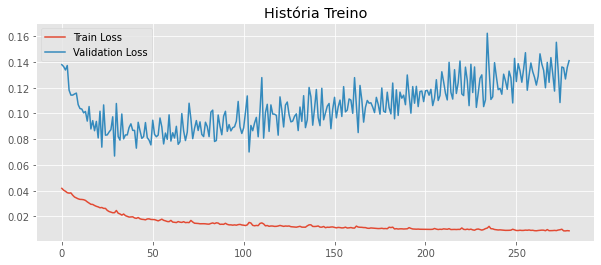
\includegraphics[width=\textwidth]{./Figuras/resultados/case1_rnn_exo_1_train.png}
        \caption{Treino do modelo RNN\_EXO\_1 na 1a fase, RMSE = 132.94} \label{fig:case1_rnn_exo_1_train} }
        \end{figure}
        \end{minipage} \hfill %
        \end{center} 
      }
     
    \paragraph{Resultados de treino e validação para a segunda fase}
    {\begin{center} \begin{minipage}[b]{1.0\textwidth}
        \begin{figure}[H]
          \center{
            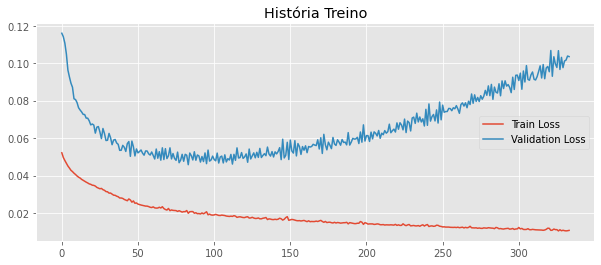
\includegraphics[width=\textwidth]{./Figuras/resultados/case2/case2_rnn_exo1_train.png}
          \caption{Gráfico de treino do modelo RNN\_EXO\_1 na 2a fase, RMSE = 109.97} \label{fig:case2_rnn_exo1_train} }
        \end{figure}\end{minipage} \hfill %
        \end{center} }
    
    \subsection{Comparativo de teste do modelo no primeiro semestre, entre as 2 fases}
        Como este modelo treinado na segunda fase obteve os melhores resultados do trabalho, foram recalculadas as métricas para o teste de modelo dentro do domínio do primeiro semestre de 2019 para realizar uma comparação justa com sua versão treinada e testada também no primeiro semestre de 2019 na primeira fase.
        
        A tabela \ref{table:case1_rnn_exo_1} demonstra que o RMSE de teste do modelo treinado na primeira fase foi notoriamente maior, e portanto pior, do que o RMSE treinado na segunda fase de acordo com a tabela \ref{table:case2_rnn_exo_2_incase1}. O RMSE sendo menor no treino deste modelo na segunda fase já trás uma melhoria em todas as outras métricas em comparação com o seu treino na primeira fase.
        A soma dos erros positivos de predições também foi menor na segunda fase, o que impacta menor em descarte de refeições.
        O RMSE deste modelo testado na primeira fase e alcançando RMSE = 106,2080 também se saiu melhor do que o melhor modelo da primeira fase, o RNN\_ENDO\_2 que alcançou RMSE = 108,06.
        
        O gráfico scatter do modelo treinado na primeira fase, conforme figura \ref{fig:case1_rnn_exo_1_test_scatter} também se saiu pior, mais distante da borda superior direita do gráfico, em relação ao scatter do modelo treinado na segunda fase conforme a figura \ref{fig:case2_rnn_exo2_test_incase1_scatter}.
        
        Por fim na comparativa entre os gráficos de predição, o modelo RNN\_EXO\_1 treinado na primeira fase produziu predições piores, e não aprendeu a sazonalidade semanal do consumo, como pode ser observado na figura \ref{fig:case1_rnn_exo_1_test}, é possível notar também, na tabela  \ref{table:case1_rnn_exo_1}, que a correlação entre os valores previstos e o consumo real, bem como o valor $R^2$ foi inferior em comparação às métricas do modelo treinado na segunda fase, e que este modelo treinado na segunda fase aprendeu melhor a sazonalidade semanal e mensal do consumo como pode ser observado na figura \ref{fig:case2_rnn_exo2_test_incase1}.
        
        \paragraph{Teste para o 1o semestre, treino na 1a fase}
            {
    	    \begin{center} 
    	        \begin{minipage}[c]{1.0\textwidth}
                  \begin{figure}[H]
                      \center{                    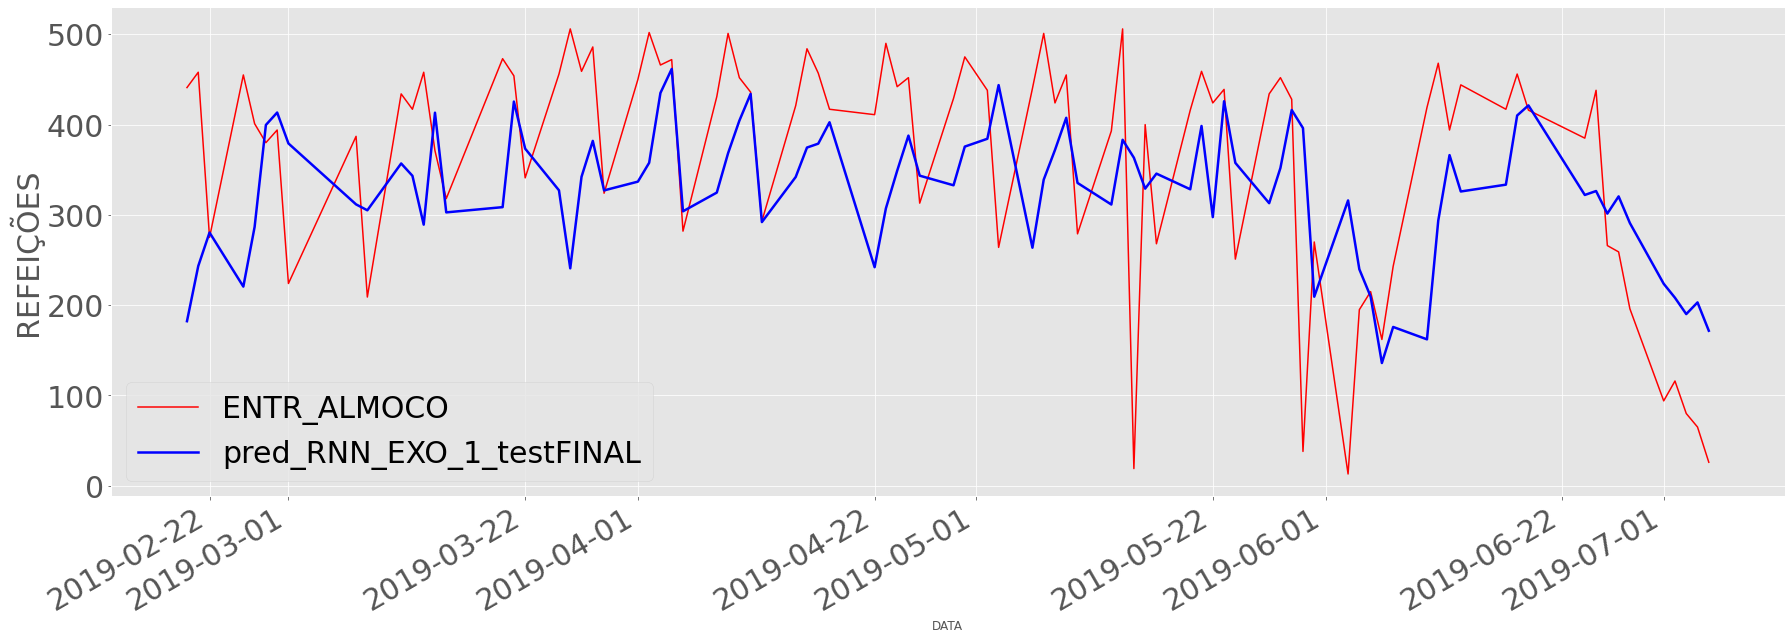
\includegraphics[width=\textwidth]{./Figuras/resultados/case1_rnn_exo_1_test.png}
                      \caption{Teste do modelo RNN\_EXO\_1, 1a fase} 
                      \label{fig:case1_rnn_exo_1_test} }
                    \end{figure} 
                \end{minipage} \hfill %
                
                \begin{minipage}[c]{0.5\textwidth}
                    \begin{figure}[H]
                      \center{                    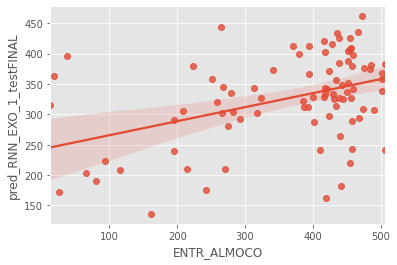
\includegraphics[width=\textwidth]{./Figuras/resultados/case1_rnn_exo_1_test_scatter.png}
                        \caption{Gráfico scatter de teste do modelo RNN\_EXO\_1, 1a fase} \label{fig:case1_rnn_exo_1_test_scatter} }
                        \end{figure}
                \end{minipage} 
            \end{center} }
            
            \begin{table}[!ht]
            \centering
            \caption{RNN\_EXO\_1 TREINADO NA 1A FASE,TESTE 1o SEMESTRE 2019}
            \label{table:case1_rnn_exo_1}
            \rowcolors{2}{gray!25}{white}
                \begin{tabular}{|c|c|}
                \rowcolor{gray!50}
                \hline
            \multicolumn{2}{c}{RNN\_EXO\_1 TREINADO NA 1A FASE,TESTE 1o SEMESTRE 2019} \\
            \hline
            RMSE & 124.49\\
            TOTAL DE REFEIÇÕES CONSUMIDAS & 31962 \\
            TOTAL DE REFEIÇÕES PROJETADAS & 28728.816  \\
            ERRO DE PREVISÃO & -3233.1839375 \\
            PERCENTAGEM DE ERRO & -10.11\%  \\
            CORRELAÇÃO (r) & 0.41 \\ 
            P-value & 6.59e-05\\ 
            R2 & 0.16\\
            SOMA DOS ERROS NEGATIVOS & -2709.17\\
            SOMA DOS ERROS POSITIVOS & 5942.35\\
            ERRO ABSOLUTO MEDIANO & 85.59\\
            ERRO ABSOLUTO PERCENTUAL MÉDIO & 90.98\% \\ \hline \end{tabular} \end{table}
        
        \paragraph{Teste para o 1o semestre, treino na 2a fase}
            \begin{table}[!ht]
            \centering
            \caption{RNN\_EXO\_1 TREINADO NA 2A FASE, TESTE 1o SEMESTRE 2019}
            \label{table:case2_rnn_exo_2_incase1}
            \rowcolors{2}{gray!25}{white}
                \begin{tabular}{|c|c|}
                \rowcolor{gray!50}
                \hline
                \multicolumn{2}{c}{RNN\_EXO\_1 TREINADO NA 2A FASE, TESTE 1o SEMESTRE 2019}\\ \hline
                RMSE & 106.2080\\
                TOTAL DE REFEIÇÕES CONSUMIDAS & 31962\\
                TOTAL DE REFEIÇÕES PROJETADAS & 32170.24\\
                ERRO DE PREVISÃO & 208.2460 \\
                PERCENTAGEM DE ERRO & 0.6515\%  \\
                CORRELAÇÃO (r)& 0.5903766574738285 \\
                P-value (p) & 1.4143e-09\\
                R2 & 0.3485\\
                SOMA DOS ERROS NEGATIVOS & -3454.8698\\
                SOMA DOS ERROS POSITIVOS & 3246.6228\\
                ERRO ABSOLUTO MEDIANO & 59.5414\\
                ERRO ABSOLUTO PERCENTUAL MÉDIO & 83.2671\% \\ \hline
            \end{tabular}
            \end{table}
            {
            \begin{center} 
            \begin{minipage}[c]{1.0\textwidth}
            \begin{figure}[H]
              \center{
                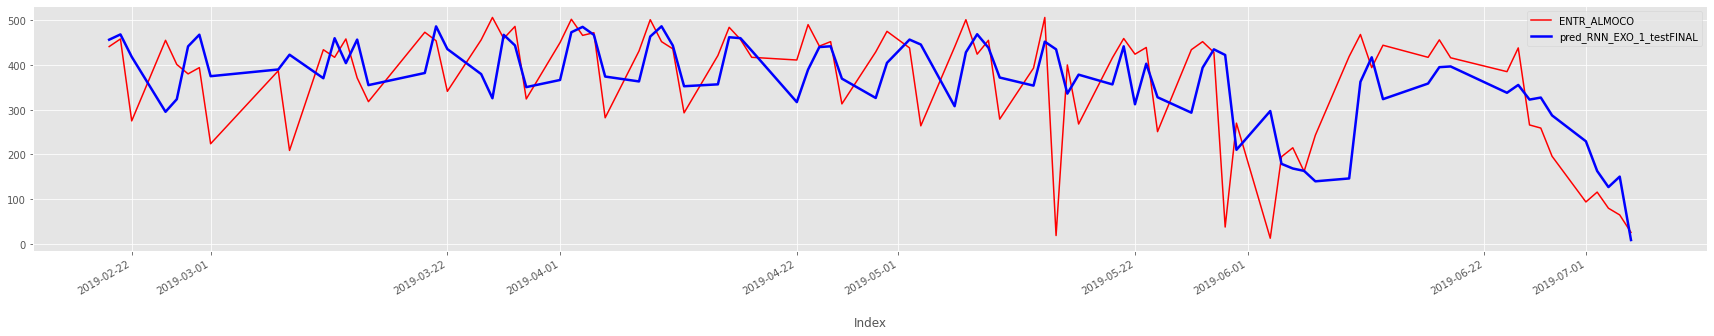
\includegraphics[width=\textwidth]{./Figuras/resultados/case2/case2_rnn_exo2_test_incase1.png}
              \caption{Gráfico teste do primeiro semestre do RNN\_EXO\_1 treinado na segunda fase} \label{fig:case2_rnn_exo2_test_incase1} }
            \end{figure}
            \end{minipage} \hfill %
            
            \begin{minipage}[c]{0.45\textwidth}
            \begin{figure}[H]
              \center{
                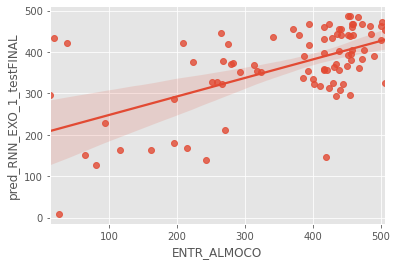
\includegraphics[width=\textwidth]{./Figuras/resultados/case2/case2_rnn_exo2_test_incase1_scatter.png}
              \caption{Gráfico scatter de teste do primeiro semestre, RNN\_EXO\_1 treinado na segunda fase} \label{fig:case2_rnn_exo2_test_incase1_scatter} }
                \end{figure}
                \end{minipage} 
                \end{center} 
            }
    \subsection{Teste final do modelo}
     O teste final do modelo RNN\_EXO\_1 por fim produziu os melhores resultados com seu treino na segunda fase e sendo testado para o ano inteiro de 2019. O RMSE observado na tabela \ref{table:case2_rnn_exo_2_2019} foi notoriamente inferior à todos os modelos treinados e testados em todo o trabalho.
     O descarte de refeições obtido pela soma dos erros positivos atingiu o valor de 4768 refeições.
     É possível notar na figura \ref{fig:case2_rnn_exo1_test} que o modelo aprendeu bem a sazonalidade mensal e semanal do consumo, mas obteve erro discrepante para o primeiro valor previsto do segundo semestre, o erro foi justificável pois seu conjunto de treino contempla apenas 1 ano com 1 alternância de semestre impossibilitando um aprendizado melhor sobre este comportamento.
     O gráfico scatter ilustrado na figura \ref{fig:case2_rnn_exo1_test_scatter} também demonstra uma boa regressão linear sobre os valores previstos pelo modelo e o valor real de consumo, se aproximando da função identidade de uma previsão ideal.
     
     {\begin{center} \begin{minipage}[c]{1.0\textwidth}
        %%% RNN_EXO_1
        \begin{figure}[H]
          \center{
            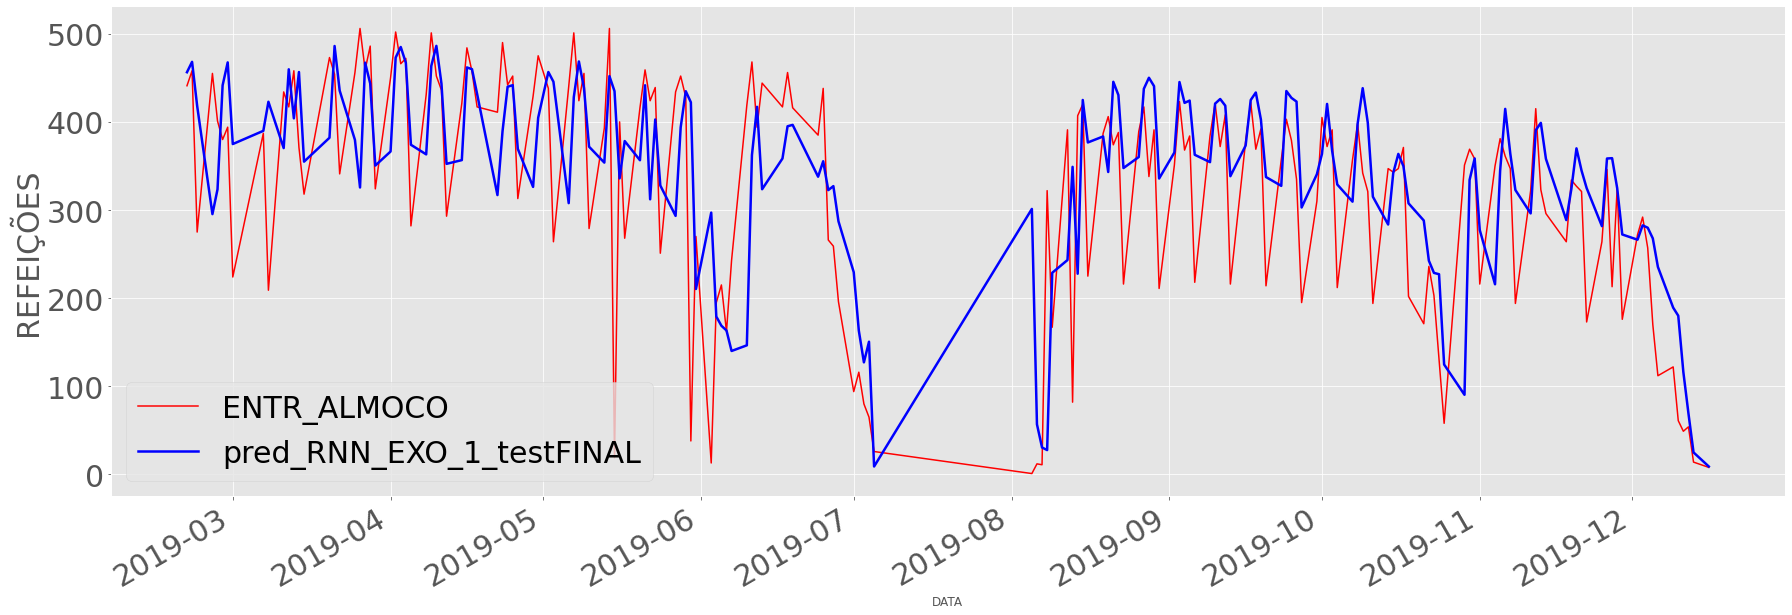
\includegraphics[width=\textwidth]{./Figuras/resultados/case2/case2_rnn_exo1_test.png}
          \caption{Gráfico final de teste do modelo RNN\_EXO\_1.} \label{fig:case2_rnn_exo1_test} }
        \end{figure}
        \end{minipage} \hfill %
         \begin{minipage}[c]{0.5\textwidth}
        \begin{figure}[H]
          \center{
            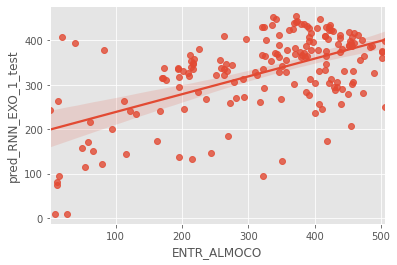
\includegraphics[width=\textwidth]{./Figuras/resultados/case2/case2_rnn_exo1_test_scatter.png}
          \caption{Gráfico de scatter do modelo  RNN\_EXO\_1.} \label{fig:case2_rnn_exo1_test_scatter} }
        \end{figure}
        \end{minipage} \end{center} }
        \begin{table}[!ht]
            \centering
            \caption{RNN\_EXO\_1 TREINADO NA 2A FASE, TESTE ANO DE 2019}
            \label{table:case2_rnn_exo_2_2019}
            \rowcolors{2}{gray!25}{white}
                \begin{tabular}{|c|c|}
                \rowcolor{gray!50}
                \hline
                \multicolumn{2}{c}{RNN\_EXO\_1 TREINADO NA 2A FASE, TESTE ANO DE 2019}\\ \hline
                RMSE & 99.36\\
                TOTAL DE REFEIÇÕES CONSUMIDAS & 58653 \\
                TOTAL DE REFEIÇÕES PROJETADAS & 62048.04\\
                ERRO DE PREVISÃO & 3395.04 \\
                PERCENTAGEM DE ERRO & 5.78\%  \\
                CORRELAÇÃO (r)& 0.67 \\
                P-value (p) & 3.29e-25\\
                R2 & 0.45\\
                SOMA DOS ERROS NEGATIVOS & -8163.18\\
                SOMA DOS ERROS POSITIVOS & 4768.13\\
                ERRO ABSOLUTO MEDIANO & 55.23\\
                ERRO ABSOLUTO PERCENTUAL MÉDIO & 83.2671\% \\ \hline
            \end{tabular}
            \end{table}


